\chapter[La biologie structurale au sein d'environnements immersifs et interactifs]{Contexte et état de l'art}
\minitoc
\cleardoublepage

\section{La biologie structurale et l'outil informatique}

\section{Réalité virtuelle et interactivité}

% \begin{eqnarray}
% \left\{ \begin{array}{ll}
% 	F_1(V\!E=0.8)=&F1 \\
% 	F_1(V\!E=0.6)=&0.925F1\\
% 	F_1(V\!E=1.0)=&1.075F1\\
% \end{array} \right.
% \end{eqnarray}

% \begin{eqnarray}
% F_1(V\!E)=
% \left\{
% 	\begin{array}{lll}
% 		&(0.7+0.375 \cdot V\!E) \cdot F1& \mbox{ si $V\!E\geq0.6$}\\
% 		&0.925 \cdot F1& \mbox{ si $V\!E<0.6$}\\
% 	\end{array}
% \right.
% \end{eqnarray}

% \begin{equation} 
% \begin{split}
% b_{TL} & = 1 - \nu + \sqrt{\nu^2-1}\\
% \nu    & = 1-\frac{1}{\eta} \\
% \eta   & = \frac{10^{TL/10}-1}{\cos(2\pi\frac{3000}{F_e})-1}
% \end{split} 
% \end{equation} 

% \begin{eqnarray} 
% \vert H( e^{2i \pi fc /F_e}) \vert = \frac{\vert H(1) \vert}{ \sqrt[]{2}}  \label{Eqa:1}
% \end{eqnarray}


% \noindent En élevant au carré (\ref{Eqa:1}), on obtient :
 
% \begin{eqnarray} 
% 	\frac{b_{TL}^2}{2 \cdot (1-b_{TL})(1-\cos(2i \pi f_c / F_e)) + b_{TL}^2} &=& \frac{1}{2}
% \end{eqnarray}



% \begin{figure}
%   \centering
%   \subfloat
%   [{\it Sans dépendance}]
%   {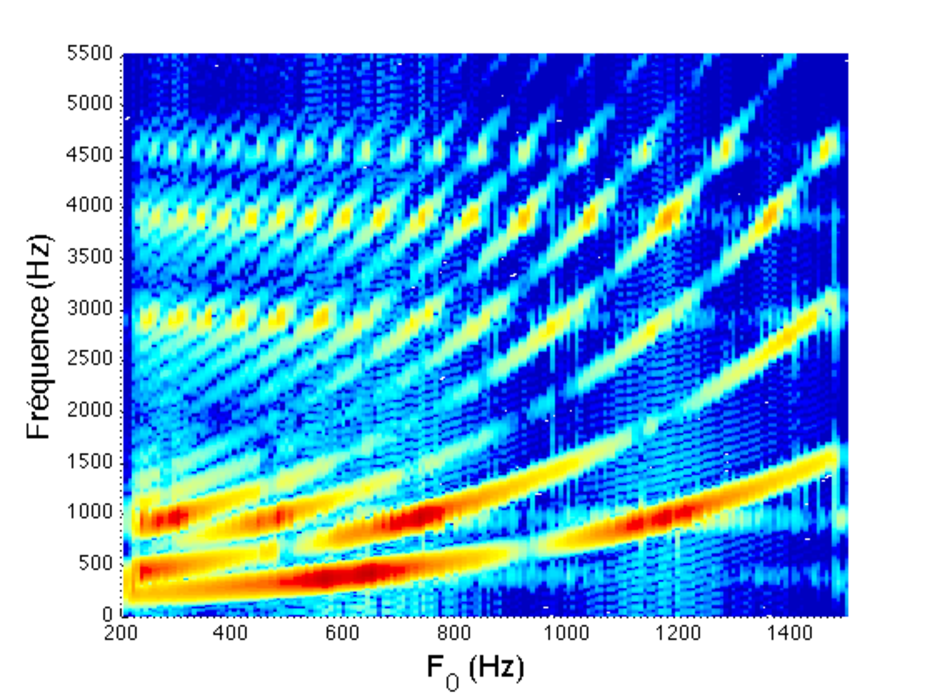
\includegraphics[width=.45\linewidth]{ch2/fig/Fi-F0-dpdce-sans_soprano_u_200-1500Hz_dig13b3.pdf}}
%   \label{Fig:Fi-F0-dpdce_sans}
%   \hspace{0.3cm}
%   \subfloat
% 	[{\it Avec dépendances}]  
%   {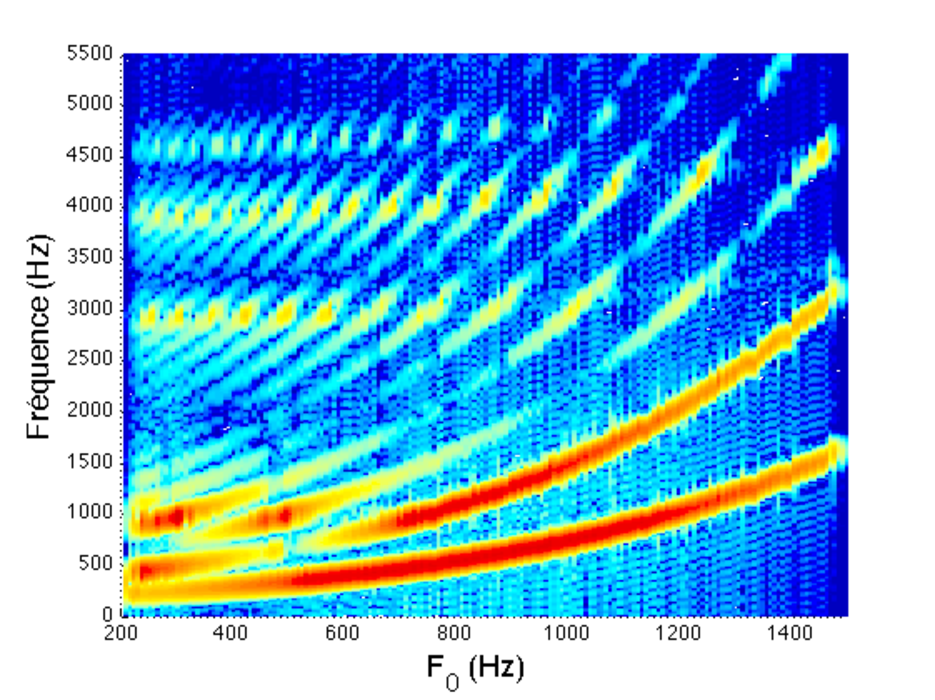
\includegraphics[width=.45\linewidth]{ch2/fig/Fi-F0-dpdce-avec_soprano_u_200-1500Hz_dig13b3.pdf}}
%   \label{Fig:Fi-F0-dpdce_avec}
%     \caption{{\it Spectrogrammes de la voyelle /a/ de synthèse, où $F_0$ augmente avec le temps, (a) sans ou (b) avec les dépendances entre les fréquences centrales des formants et de $F_0$. \textit{Voir fichiers audios~/ vidéos~\ref{fav:fi-f0-dependance}}\\
% }}
%   \label{Fig:Fi-F0-dpdce}
% \end{figure}

% \subsubsection{a) La soufflerie}

% \begin{table}[!h]
% 	\centering
% 	\begin{tabular}{|c|c|c|} 
% 		\hline
% 		& \centering \textbf{Tessiture naturelle moyenne} & \centering \textbf{Tessiture
% dans le synthétiseur} \tabularnewline
% 		\hline
% 		\bf Basse & Mi2-Mi4 & Sol$\sharp$1-Sol4\\
% 		\hline
% 		\bf Ténor & Do3-Si4 & Sol$\sharp$1-Sol4\\
% 		\hline
% 		\bf Alto & Fa3-Mi5 & Sol$\sharp$2-Sol5\\
% 		\hline
% 		\bf Soprano & Si3-Do6 & Sol$\sharp$3-Sol6\\
% 		\hline
% 	\end{tabular}
% 	\caption{\textit{Tessiture des chanteurs naturels et synthétiques (La3=440 Hz). Voir fichiers audios~/ vidéos~\ref{fav:types-voix-1}}}
% 	\label{Tab:tessChant}
% \end{table}

